% appendix.tex -- en (English)
The appendix contains EAGLE drawings of the additional TinkerKit board:
\begin{compactitem}
	\item Wiring conception of the TinkerKit push buttons
	\item schematic of the TinkerKit board
	\item printed circuit board
	\begin{compactitem}
		\item dimensions
		\item top side
		\item bottom side
	\end{compactitem}
%	\item Placement (mounting) of components
\end{compactitem}

\section{Assembling Variants}
The printed circuit board may be assembled in such a way that it
corresponds functionally to the prototype described in section
\ref{sect:TinkerKitBoard}.
An alternative assembly of the board provides six pushbuttons
distinguishable by voltage dividers at the analogue inputs of the white
TinkerKit connectors. At the digital inputs of the orange TinkerKit
connectors there can be connected two further external pushbuttons. They
can be mounted elsewhere at the {\Bezeichnung} (e.g. as shoulder buttons
on the housing).

Table \ref{tab:variants} shows the corresponding assembly variant of
each version:

\begin{table}[h]
\centering
\renewcommand{\arraystretch}{1.5}
\begin{tabular}{|p{0.24\textwidth}|p{0.16\textwidth}|p{0.18\textwidth}|p{0.15\textwidth}|p{0.16\textwidth}|}
\hline
\textbf{version}										&	\textbf{RDIG\_ORL, RDIG\_ORR}	&	\textbf{RANA\_ORL, RANA\_ORR}	&	\textbf{RDN\_ORL, RDN\_ORR}	&	\textbf{RDN\_PINL, RDN\_PINR}\\
\hline
	four analogue buttons,\newline two digital buttons	&	0R								&	not mounted						&	1k							&	not mounted\\
\hline
	six analogue buttons,\newline two external buttons	&	not mounted						&	0R								&	68k or 82k (t.b.d.)			&	1k\\
\hline
\end{tabular}
\vspace{0.5cm}
\caption{Assembly Variants}
\label{tab:variants}
\end{table}




%---------------------------------------------------------------
%  conception
%---------------------------------------------------------------
%%%%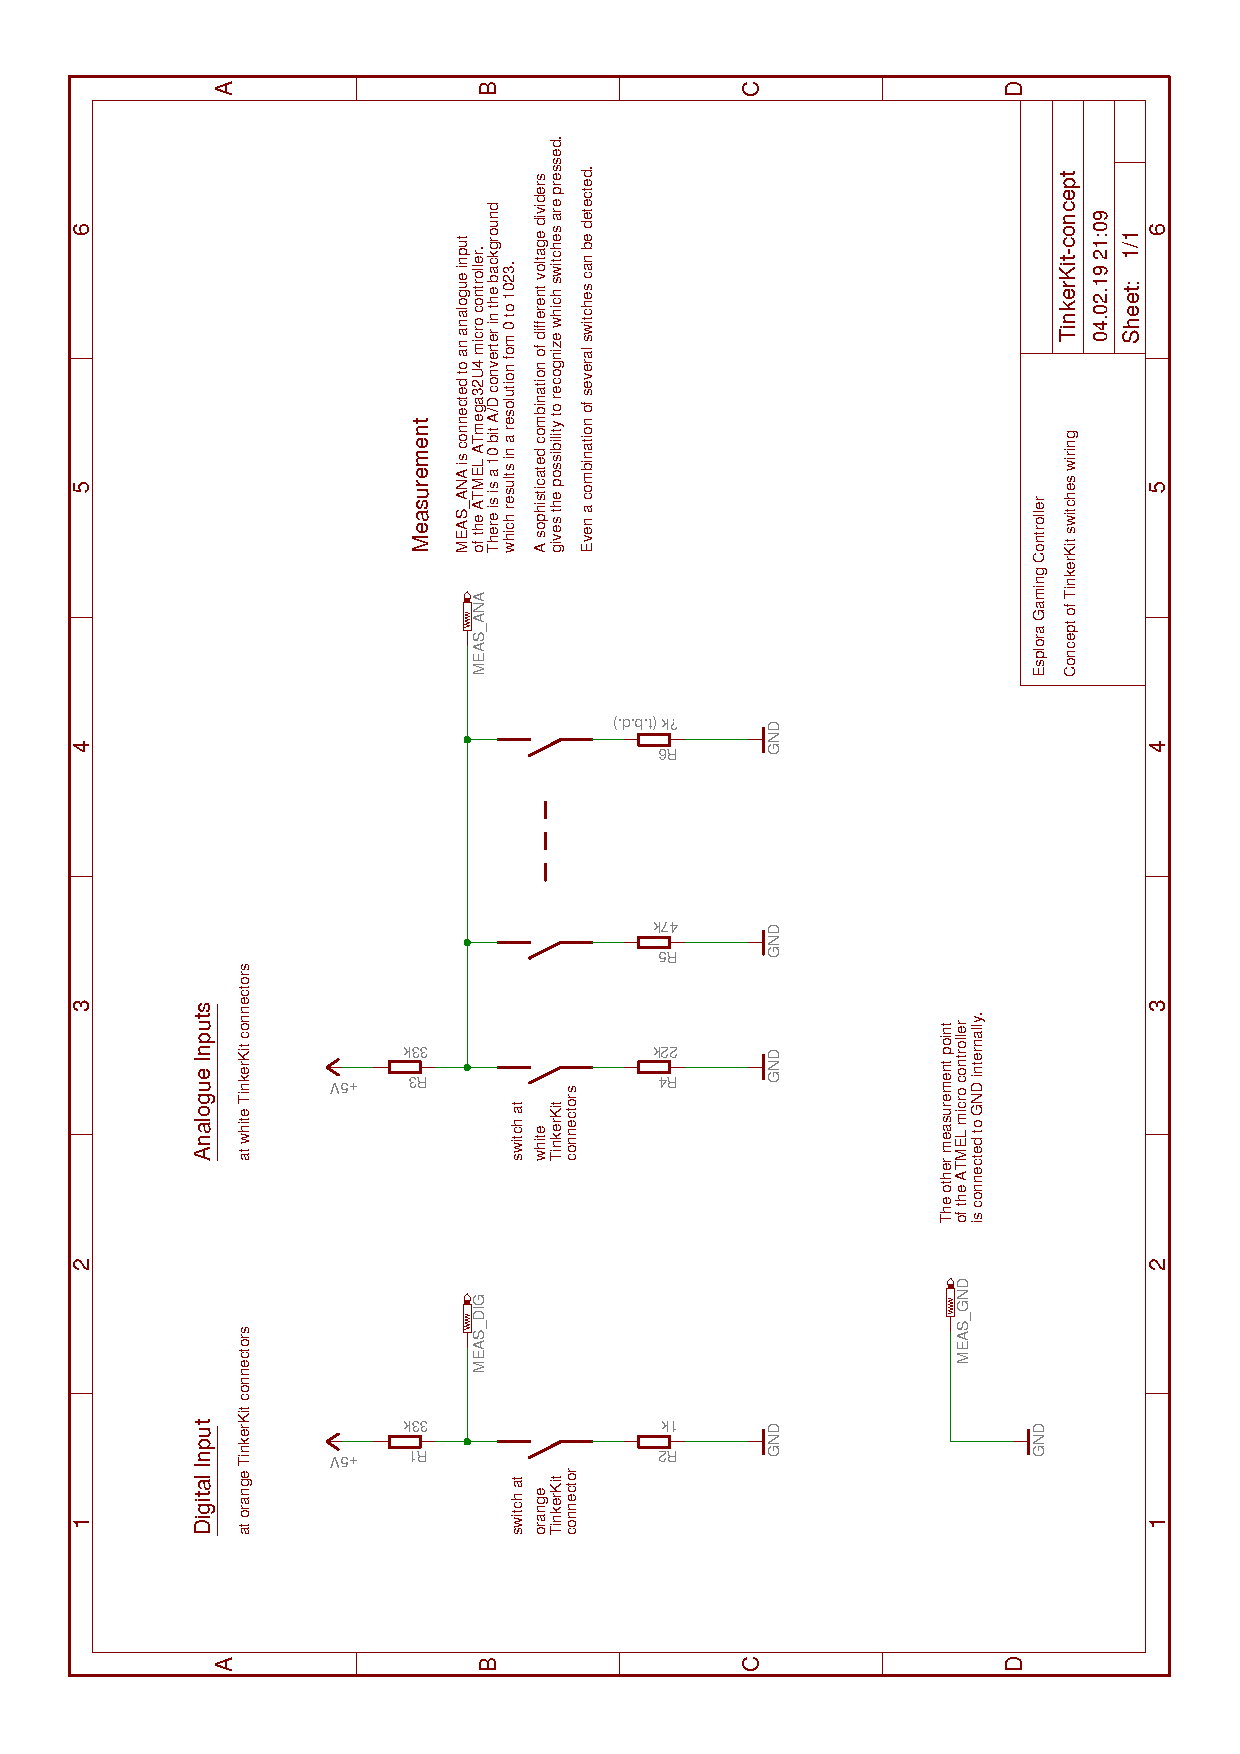
\includepdf[pages=-, portrait, scale=1.0, addtotoc={1,section,0,Konzept,Konzept} ]{./pics/eagle/TinkerKit-concept.pdf}
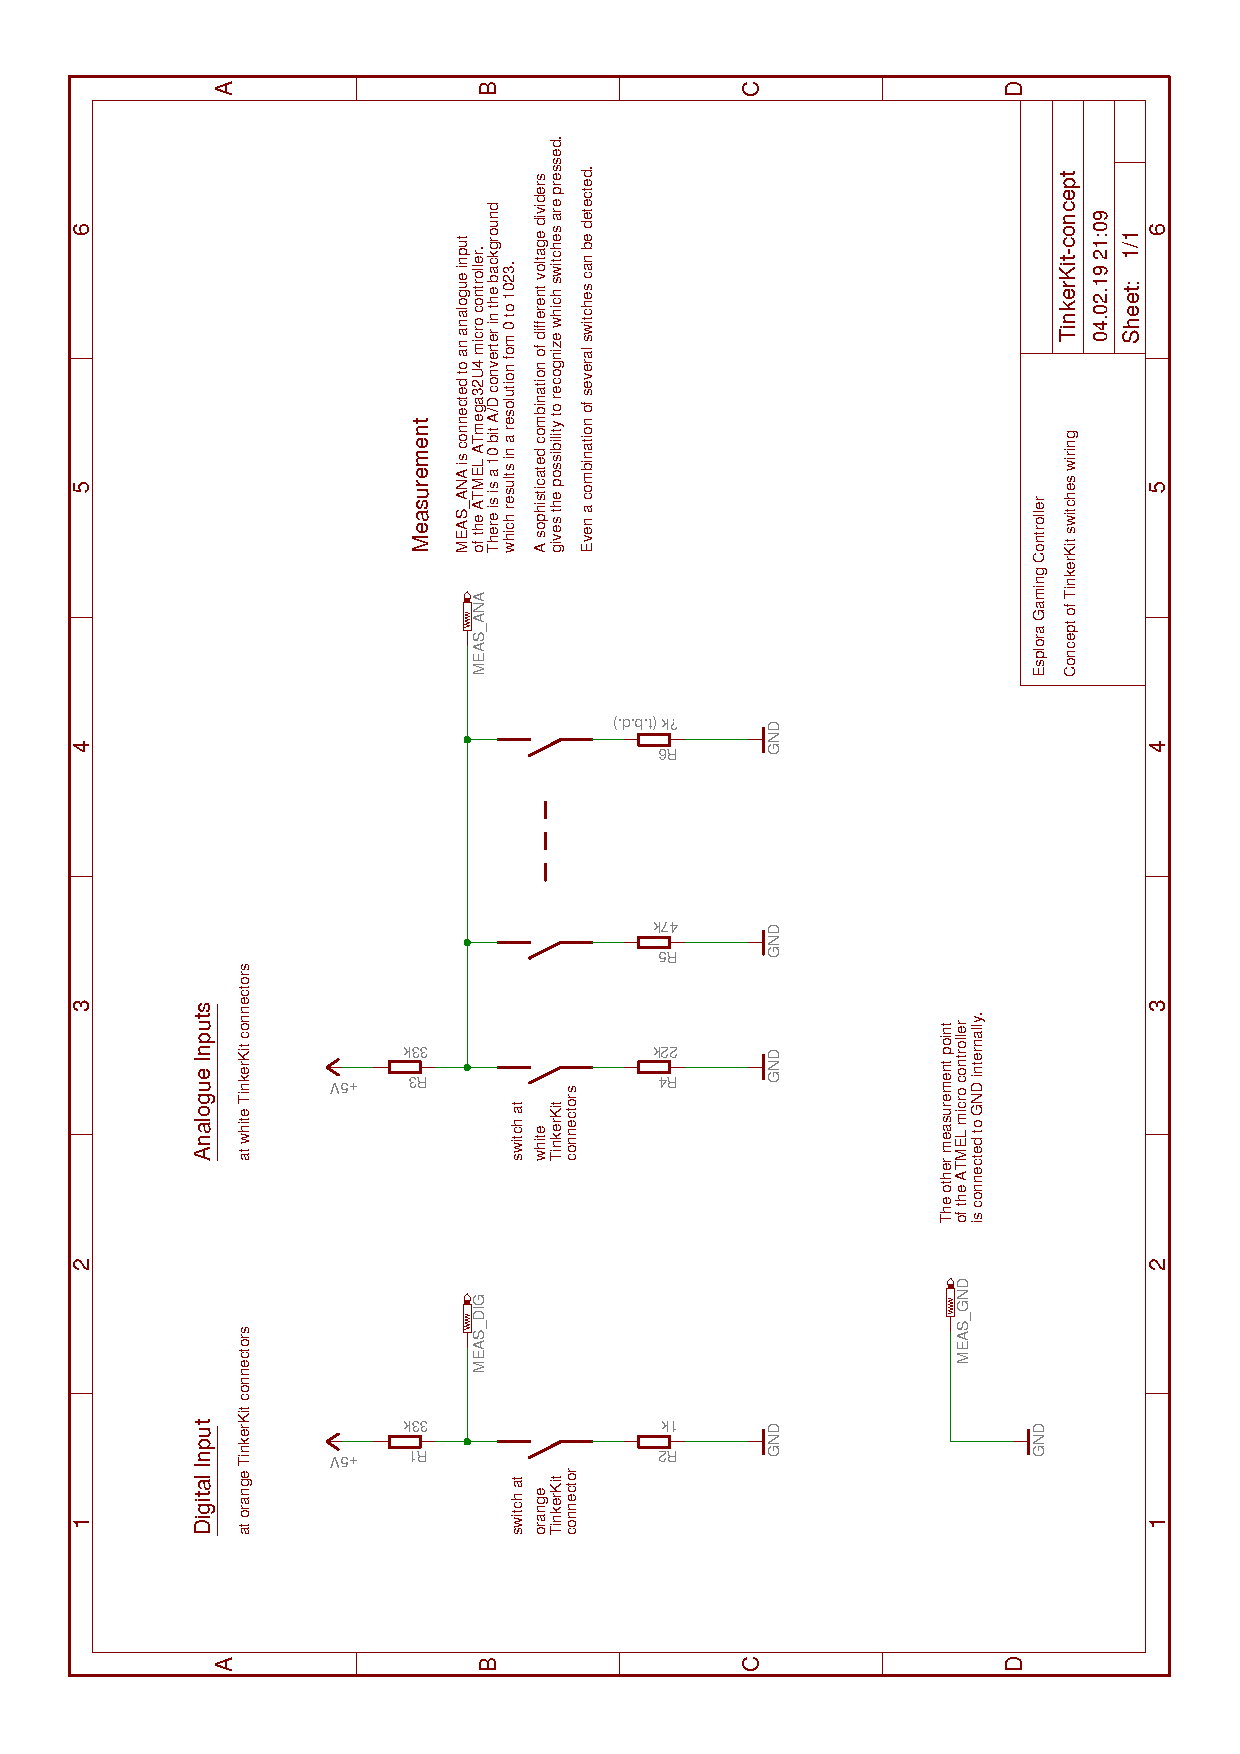
\includepdf[pages=-, , scale=1.0, addtotoc={1,section,0,Conception,Conception} ]{./pics/eagle/TinkerKit-concept.pdf}

%---------------------------------------------------------------
%  schematics
%---------------------------------------------------------------
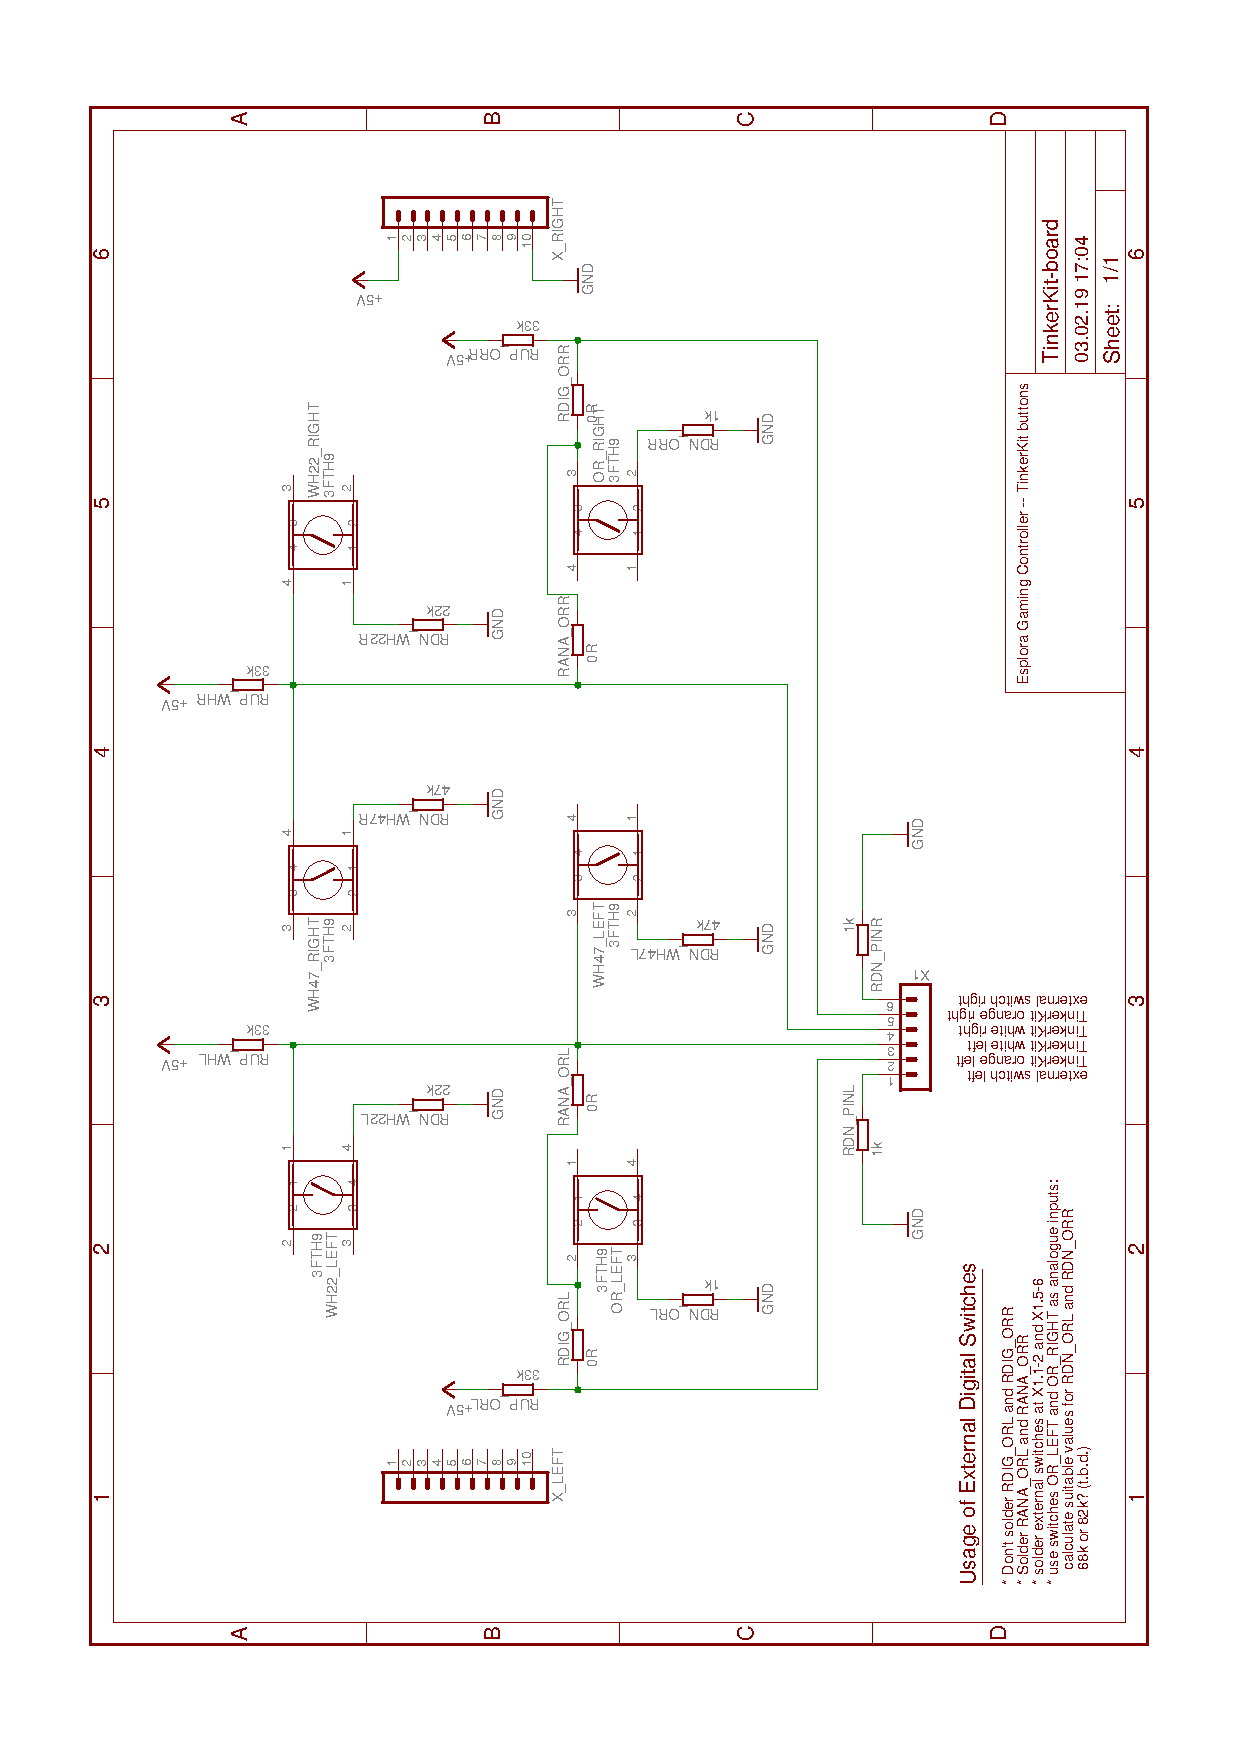
\includepdf[pages=-, , scale=1.0, addtotoc={1,section,0,TinkerKit Board Schematics,TinkerKit Board Schematics} ]{./pics/eagle/TinkerKit-board_SCH.pdf}

%---------------------------------------------------------------
%  PCB
%---------------------------------------------------------------
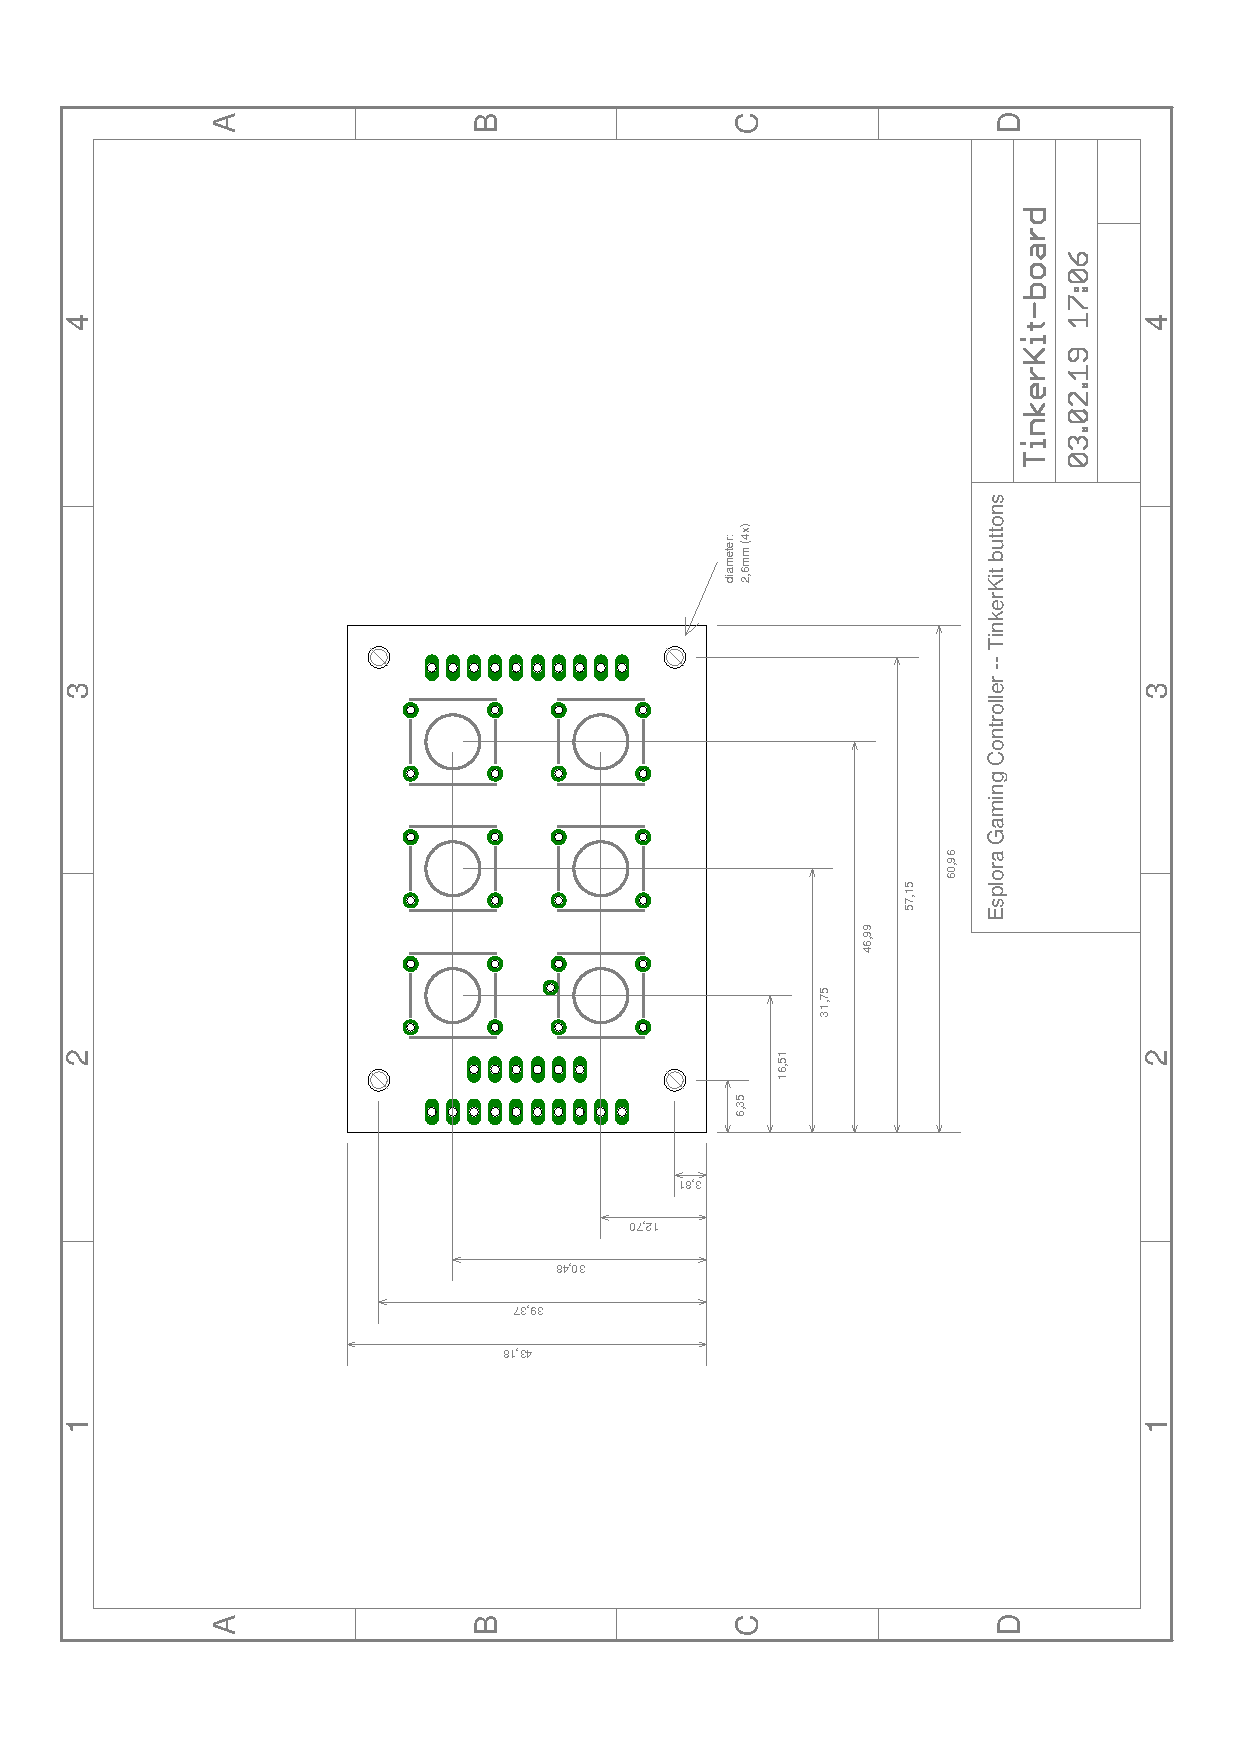
\includepdf[pages=-, , scale=1.0, addtotoc={1,section,0,TinkerKit Board Dimensions,TinkerKit Board Dimensions} ]{./pics/eagle/TinkerKit-board_MEAS.pdf}
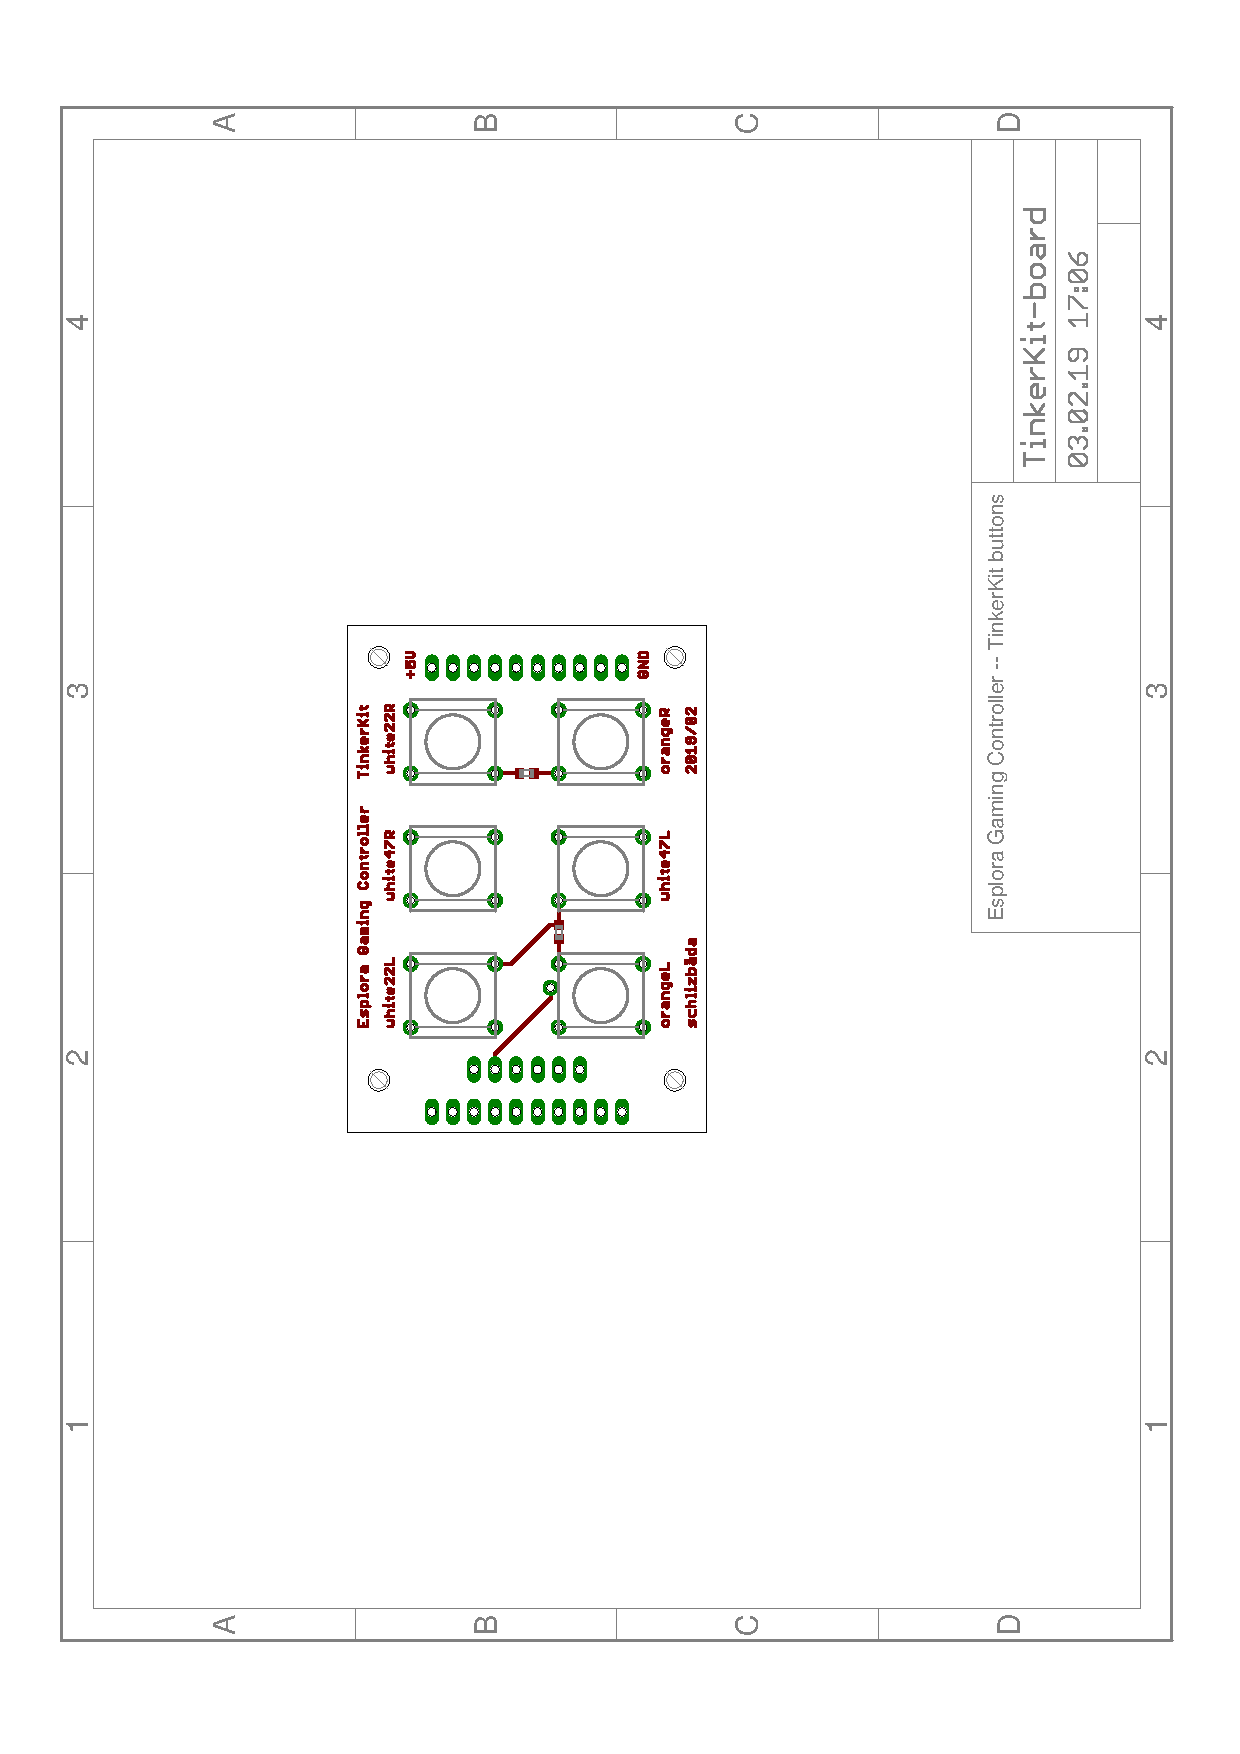
\includepdf[pages=-, , scale=1.0, addtotoc={1,section,0,TinkerKit Board Top Side,TinkerKit Board Top Side} ]{./pics/eagle/TinkerKit-board_TOP.pdf}
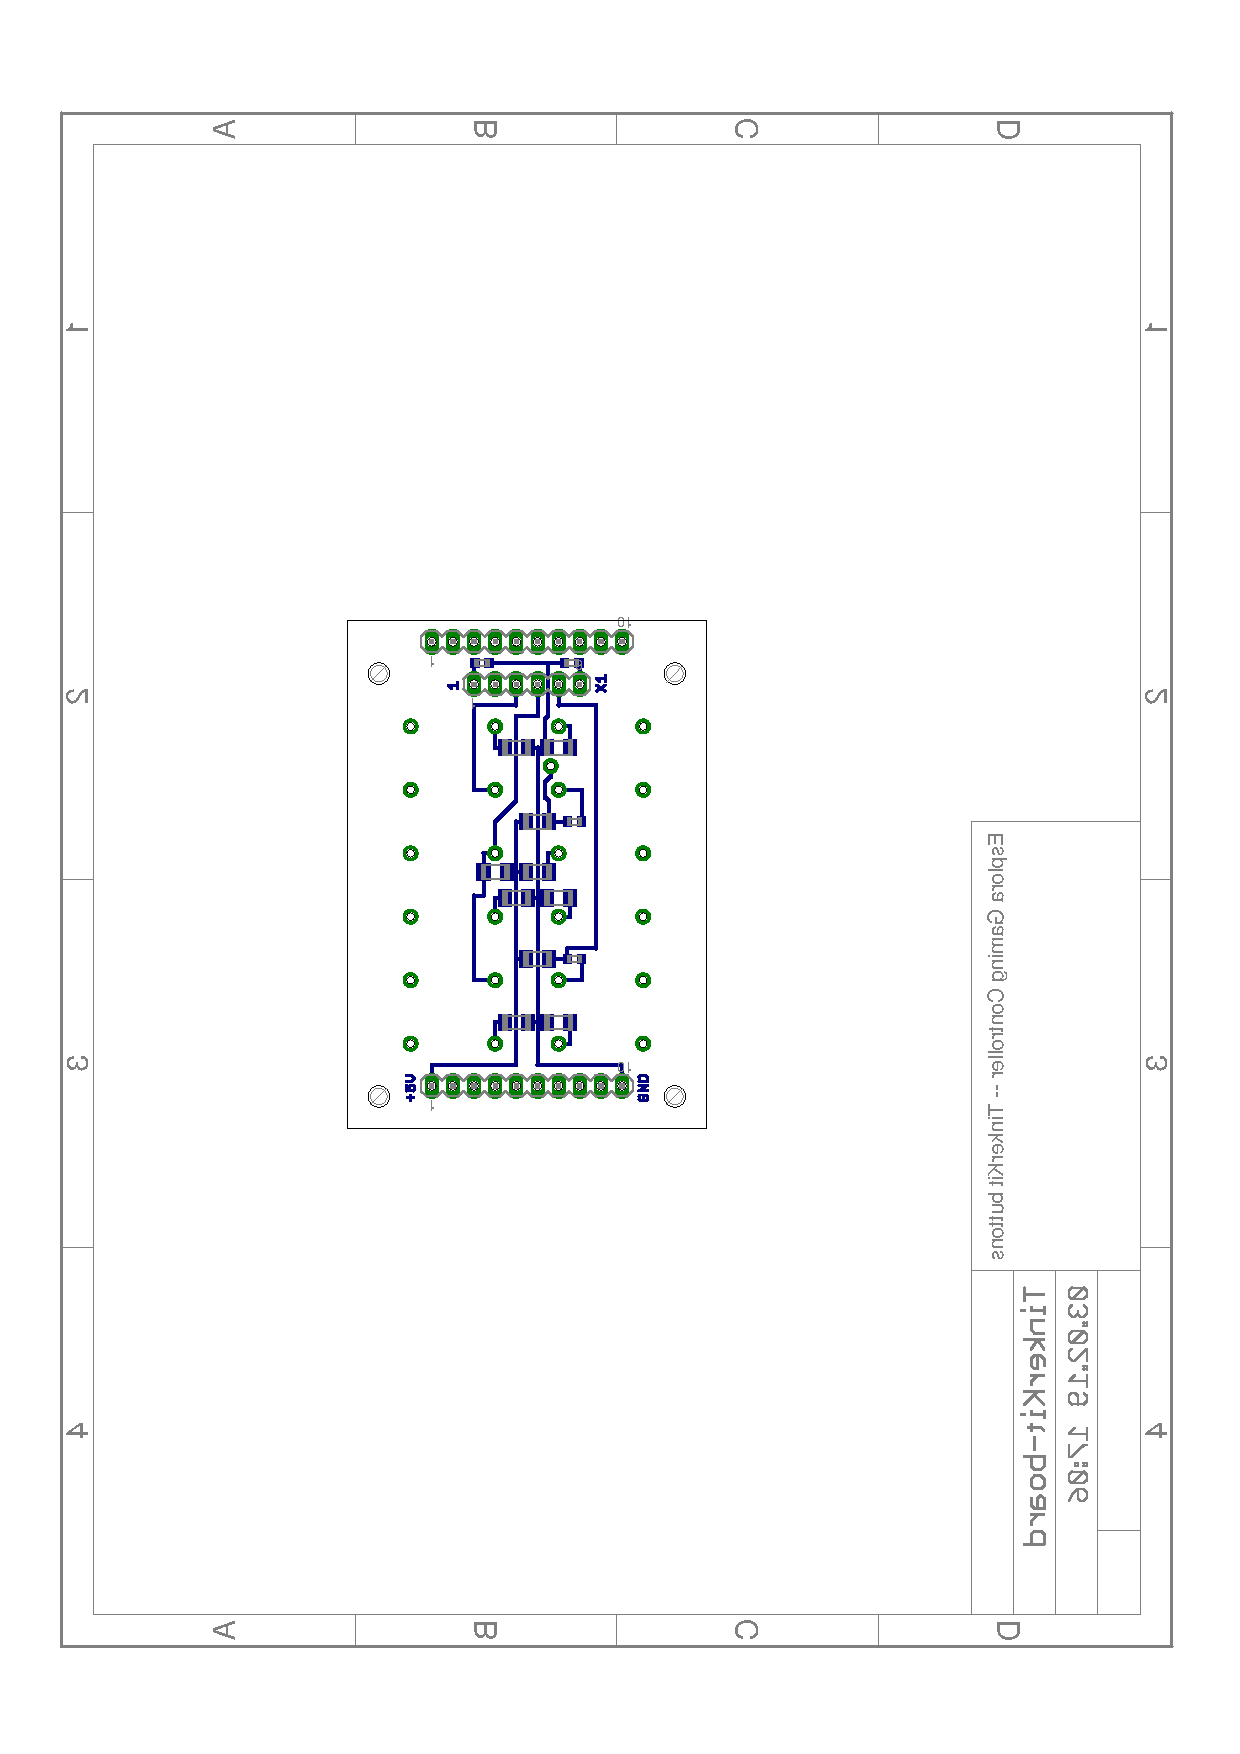
\includepdf[pages=-, , scale=1.0, addtotoc={1,section,0,TinkerKit Board Bottom Side,TinkerKit Board Bottom Side} ]{./pics/eagle/TinkerKit-board_BOT.pdf}

%%---------------------------------------------------------------
%%  parts
%%---------------------------------------------------------------
%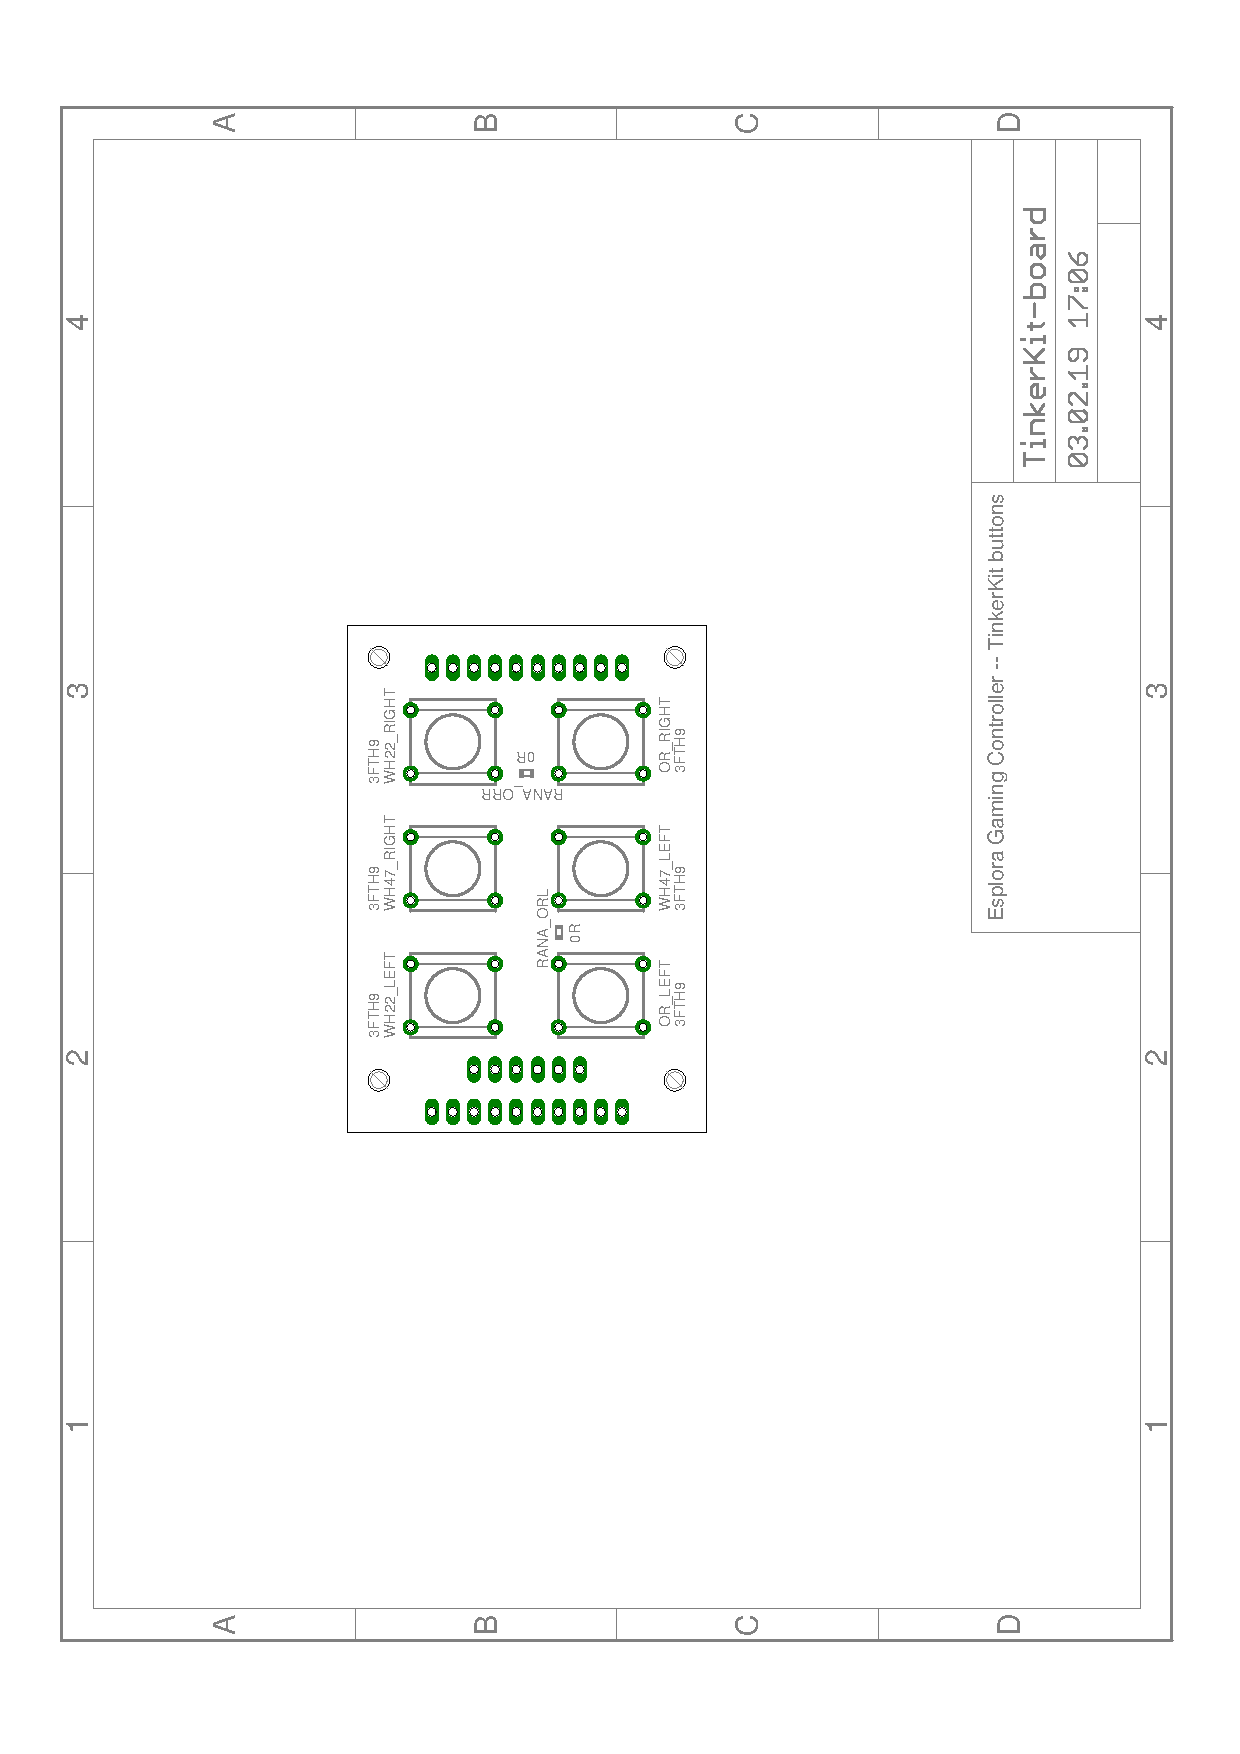
\includepdf[pages=-, , scale=1.0, addtotoc={1,section,0,Leiterplatte,Leiterplatte} ]{./pics/eagle/TinkerKit-board_TOPparts.pdf}
%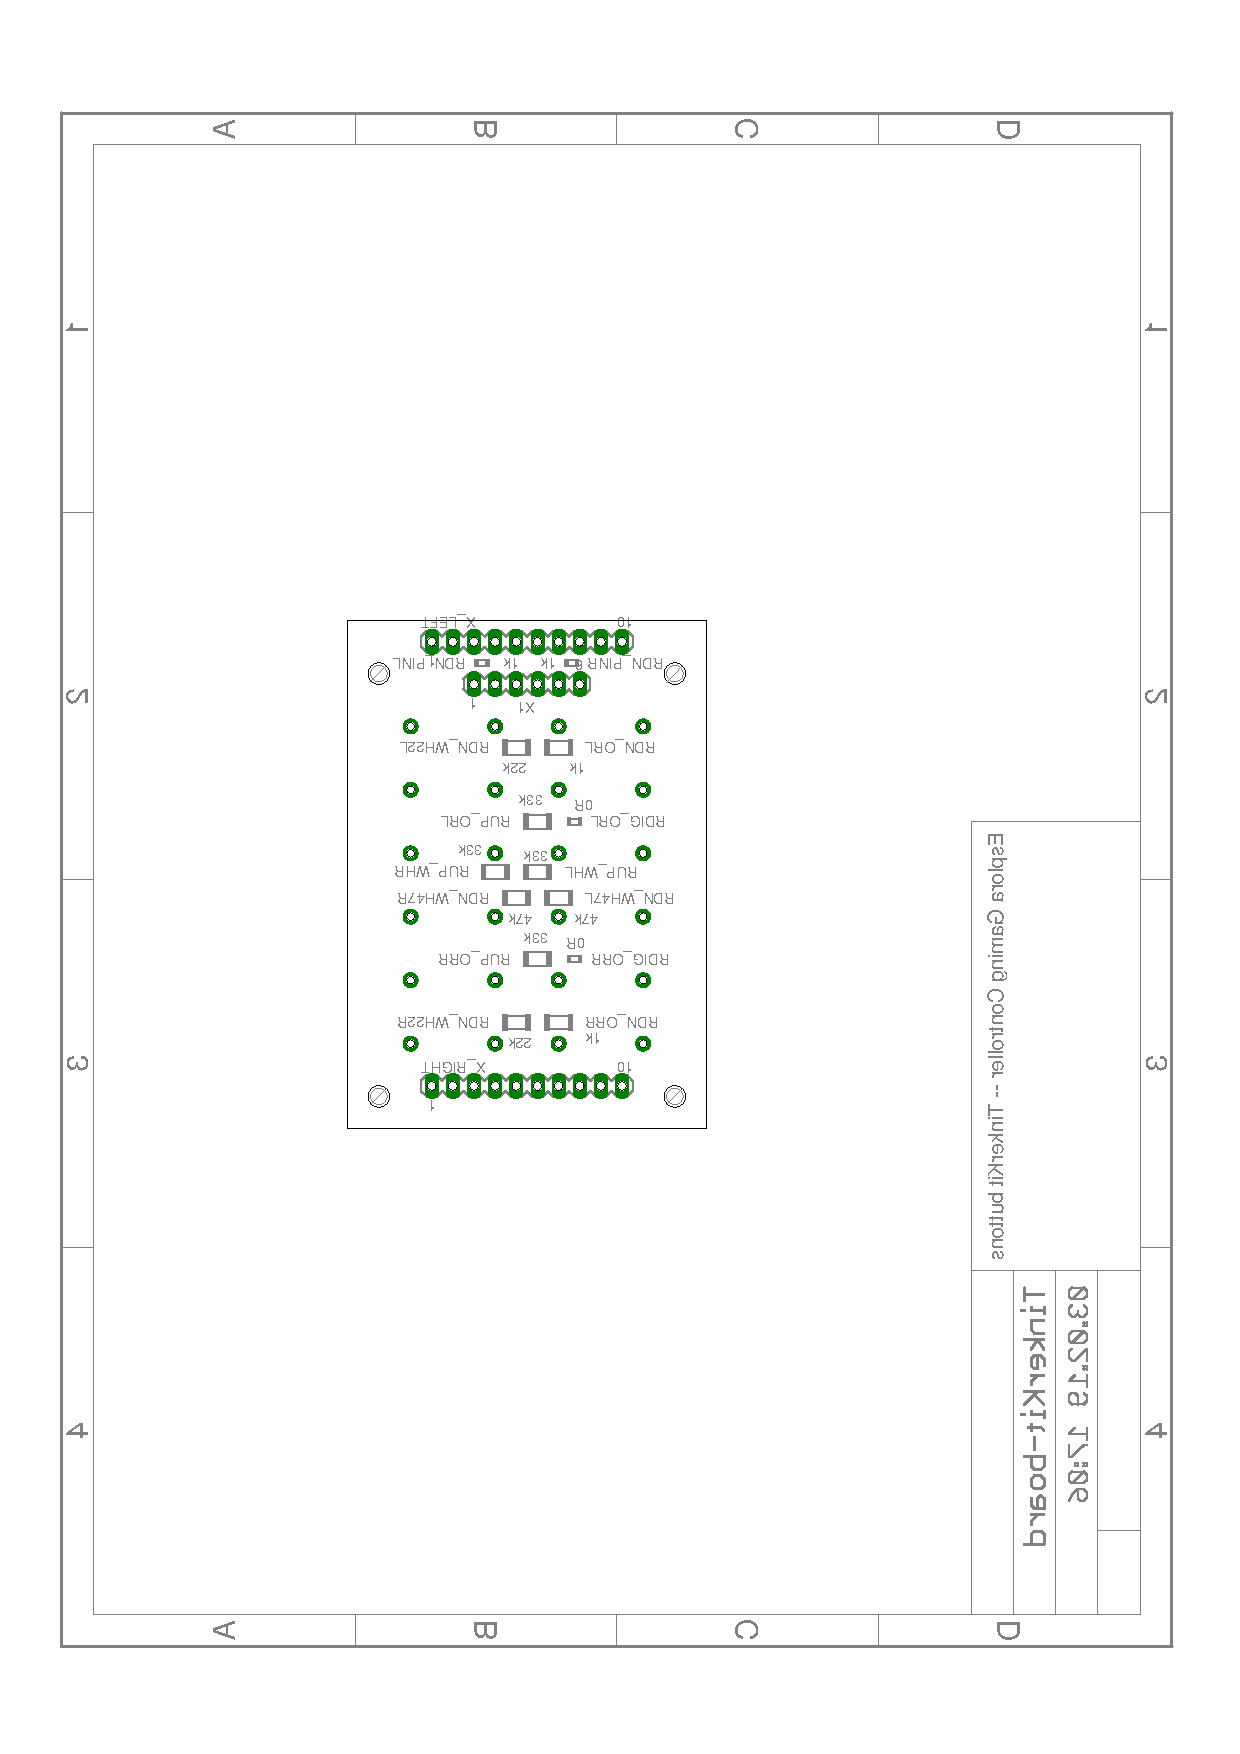
\includepdf[pages=-, , scale=1.0, addtotoc={1,section,0,Leiterplatte,Leiterplatte} ]{./pics/eagle/TinkerKit-board_BOTparts.pdf}
